\section{Optimierungsverfahren}
% TODO: Begriff "Konvergenz" im ersten paragrah erklären, dann in metaheuristiken in Relation stellen zu diversifizierung und intensivierung und in hybride heuristiken als motivation aufgreifen!

% TODO: Einordnung von Evolutionären Algorithmen innerhalb der Metaheuristiken spezifizieren (populationsbasiert und stochastisch) (in zweiter Grafik) ggf Beispiele für andere Kategorien anführen

Im vorherigen Abschnitt haben wir uns unter anderem damit befasst wie die Parameter eines HMMs mittels des Baum-Welch Algorithmus optimiert werden können. In diesem Kapitel treten wir einen Schritt zurück und beantworten die Fragen was es überhaupt bedeutet Dinge zu optimieren und welche verschiedenen Optimierungsansätze existieren.

\subsection{Was ist Optimierung}
Wir sprechen von einem \textbf{Optimierungsproblem} wenn wir optimale Parameter eines Systems bestimmen wollen. Als Optimale Parameter bezeichnen wir solche, die eine Problemspezifische \textbf{Zielfunktion} $f$ minimieren (oder maximieren). Die Domäne der Zielfunktion nennt man einen \textbf{Suchraum} $S$. Der Wert der Zielfunktion für eine Kombination von Parametern aus dem Suchraum gibt die \textbf{Qualität} dieser Parameter an. Oft gibt es Einschränkungen für die Parameter, so dass nicht alle Werte des Suchraumes mögliche Lösungen sind. Den Raum aller möglichen Lösungen nennen wir \textbf{zulässige Region} \cite*{MetaheuristicsEGT}.

Um diese Konzepte zu verdeutlichen betrachten wir das bekannte Problem des Handlungsreisenden (traveling salesman problem), in welchem es darum geht den Besuch mehrerer Städte optimal zu planen, so dass jede Stadt außer dem Starpunkt nur einmal besucht wird und der Endpunkt equivalent zu dem Startpunkt ist. Der Suchraum ist in diesem Fall gegeben durch alle möglichen Routen (Kombinationen der zu besuchenden Städte). Die Zielfunktion, welche wir minimieren wollen gibt die gesamte Länge einer Reiseroute an. In der zulässigen Region des Suchraumes befinden sich ausschließlich Routen in welchen jede Stadt, bis auf den Startpunkt, einmal besucht wird und der Endpunkt equivalent zum Startpunkt ist. Da Teleportation noch nicht erfunden wurde ist die zulässige Region zusätzlich eingeschränkt auf alle Routen in welchen nacheinander besuchte Städte durch eine Strecke verbunden sind.

\subsection{Kategorien von Optimierungsverfahren}
Eine Optimierungsmethode, welche stets die global optimale Lösung findet nennt man eine \textbf{exakte Methode}. Für viele Probleme gibt es jedoch keine exakten Algorithmen die eine Lösung in polynomieller Zeit finden. In solch einem Fall kann man zu einer \textbf{Heuristik} greifen. Eine Heuristik liefert eine Lösung die "gut genug" ist in "annehmbarer Zeit". Es handelt sich also um ein Verfahren, welches man umgangssprachlich als Faustregel bezeichnen würde. Eine Heuristik ist nicht das selbe wie ein \textbf{Approximationsalgorithmus}. Denn ein Approximationsalgorithmus garantiert eine untere Schranke für die Qualität einer gefundenen Lösung. Bei einer Heuristik verhält es sich ähnlich wie mit Privatkäufen über Kleinanzeigenportale: Es besteht keine Garantie. Die gefundenen Lösungen eines heuristischen Verfahrens können also beliebig schlecht sein. Heuristiken werden unterteilt in \textbf{spezifische Heuristiken} und \textbf{Metaheuristiken}. Spezifische Heuristiken sind, wie der Name bereits vermuten lässt zugeschnitten auf ein spezifisches Problem, wohingegen Metaheuristiken sehr allgemein sind und auf fast alle Optimierungsprobleme angewendet werden können \cite*{MetaheuristicsEGT}. Metaheuristiken kann man weiter unterteilen in 

Die wahrscheinlich bekannteste Heuristik ist eine \textbf{lokale Suche}. Der Baum-Welch Algorithmus zum Beispiel ist eine lokale Suche. Genetische Algorithmen, mit welchen wir uns später im Detail beschäftigen zählen zu den bekanntesten und ältesten Metaheuristiken.

Figur \ref{fig:optimierungsverfahren} zeigt die zuvor beschriebene Unterteilung der Optimierungsverfahren. Es sei angemerkt, dass die unternommene Unterteilung keineswegs Anspruch auf Vollständigkeit erhebt, sondern primär zur Einordnung des Baum-Welch Algorithmus und des genetischen Algorithmus im Kontext der Optimierungsverfahren dient.
\begin{figure}[h!]
    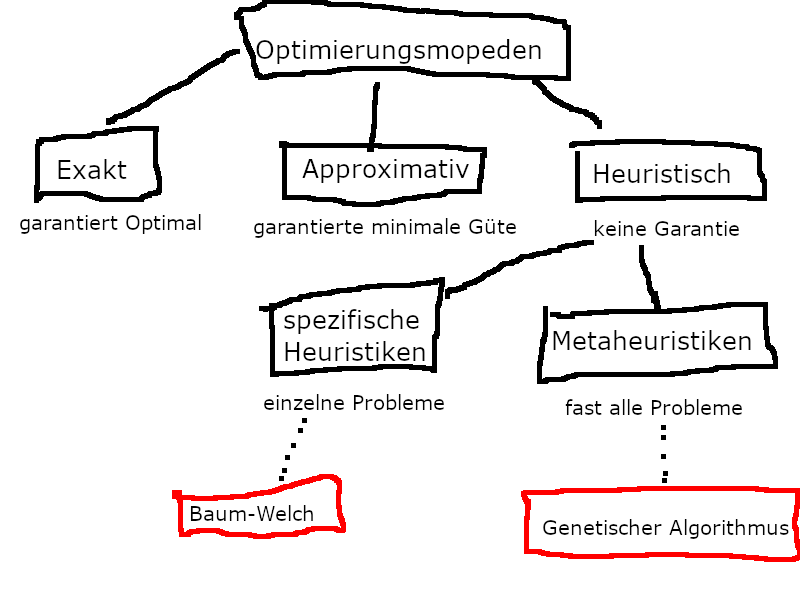
\includegraphics[scale=1.0]{images/Unterteilung_Optimierungsverfahren.png}
    \caption{Unterteilung der Optimierungsverfahren}
    \label{fig:optimierungsverfahren}
\end{figure}

\subsection{Metaheuristiken}
Bei einer Metaheuristik handelt es sich nicht um einen bestimmten Algorithmus sondern vielmehr eine Ansammlung von Ideen, Konzepten und Operatoren, welche verwendet werden können um einen spezifischen heuristischen Algorithmus zu erstellen \cite*{MetaheuristicsExposed}. Es gibt also zum Beispiel nicht \textit{den} genetischen Algorithmus sondern es existiert ein Genetischer Algorithmus "Bauplan" an welchem man sich orientieren kann.

Um eine Metaheuristik zu erstellen gilt es zwei konfliktierende Kriterien zu balancieren. Zum einen die \textbf{Diversifizierung} (exploration): das entdecken neuer Lösungen und zum anderen die \textbf{Intensivierung} (exploitation): das verbessern einer bekannten Lösung \cite*{MetaheuristicsEGT}. Reine Diversifizierung ist das selbe wie eine zufällige Suche und reine Intensivierung ist equivalent zu einer lokalen Suche.

Metaheuristiken sind oft inspiriert durch natürliche Prozesse. Bekannte Metaheuristiken aus dem Gebiet der Biologie sind \textbf{Genetische Algorithmen (GA)}, welche die Evolution einer Population durch natürliche Selektion nachahmen und \textbf{Ant Colony Optimization (ACO)} Algorithmen, welche der Pheromon-basierten Kommunikation von Ameisen innerhalb einer Kolonie nachempfunden sind. Zu den bekanntesten Beispielen aus der Physik zählt das \textbf{Simulated Annealing (SA)} Verfahren, welches angelehnt ist an den Abkühlungsprozess eines Metalls nach dem erhitzen \cite*{metaheuristics}.

\subsection{Hybride Heuristiken}
Eine kombination mehrerer verschiedener Algorithmen zu einem neuen nennt man Hybridisierung. Das kombinieren von metaheuristischen Algorithmen ist ein aktives Forschungsfeld und es existiert mittlerweile eine beachtliche Anzahl hybrider Metaheuristiken. Das kombinieren von Konzepten erlaubt es Wissenschaftlern außerhalb der Grenzen einer bestimmten Metaheuristik zu denken und ihrer Kreativität freien Lauf zu lassen \cite*{MetaheuristicsSurvey}.

Es gibt verschiedene möglichkeiten der Hybridisierung. Wenn man verschiedene Heuristiken sequentiell hintereinander ausführt spricht man von einer \textbf{Relay Hybridization (RH)}. Eine Hybridisierung in der verschiedene Heuristiken kooperativ zusammenarbeiten nennt man eine \textbf{Teamwork Hybridization (TH)} \cite*{MetaheuristicsEGT}. 

Die Hauptmotivation hinter der hybridisierung ist es komplementäre Eigenschaften verschiedener Algorithmen auszunutzen \cite*{MetaheuristicsSurvey}. Populationsbasierte Metaheuristiken, wie zum Beispiel genetische Algorithmen sind gut im diversifizieren aber schlecht im intensivieren. Eine lokale Suche wiederum ist gut im intensivieren einer Lösung, bietet aber keine Diversifizierung. Es bietet sich also an Eine populationsbasierte Metaheuristik mit einer lokalen Suche zu kombinieren \cite*{MetaheuristicsEGT}.

\subsection{Parameter Tuning}
Ein großer Nachteil vom Metaheuristiken ist, dass sie neue Parameter einführen, welche selbst optimiert werden müssen. Beispiele für solche Parameter sind die Mutationsrate eines Genetischen Algorithmus, die initiale Temperatur beim simulated annealing oder auch die Pheromonpersistenz eines Ant Colony Algorithmus. Eine Optimale Belegung dieser Parameter ist Problemabhängig. Daher gibt es keine Metaheuristik für welche universal optimale Parameter existieren. Man unterscheidet zwischen dem \textbf{Off-Line} und dem \textbf{On-Line} Parameter Tuning. In einem Off-Line Ansatz werden Werte für die Parameter vor der Ausführung des Algorithmus fixiert. Beim On-Line Parameter Tuning werden die Parameter während der Ausführung dynamisch angepasst \cite*{MetaheuristicsEGT}.

\subsection{Kritik an metapher basierten Metaheuristiken}
In den letzten Jahren wurde das Feld der Optimierung regelrecht überschwemmt mit "neuen" Metapher basierten Algorithmen. Ob Mikrofledermaus, Jazz-Musiker, Schwarze Löcher oder auch intelligente Wassertropfen. Jedes erdenkliche Konzept kann in einen Optimierungsalgorithmus verwandelt werden. Oft stellt sich jedoch heraus dass das einzige was diese "neuen" Algorithmen zum Feld beitragen eine Umbenennung eines bereits etablierten Algorithmus ist.~\cite*{NoNovelty} So ist zum Beispiel Harmony search, ein Suchalgorithmus der auf dem Prinzip von Jazz-Musikern funktioniert nichts weiteres als eine Umbenennung eines speziellen Falles des Genetischen Algorithmus.~\cite*{HarmonySearch} Trotz mangelnder Innovation verzeichnet eine Suche nach "harmony search" auf Google Scholar laut Weyland im Jahre 2010 586 Einträge. Im Jahre 2023 ist diese Zahl auf stolze 57.500 Einträge gestiegen, wovon 7.840 Einträge nach 2022 erschienen. Die Flut solcher vermeintlich "neuen" Algorithmen ist sehr nachteilig für das Feld der Optimierung, denn die elaborierten Metaphern für bereits existierende Konzepte führen zu Verwirrung und tatsächlich innovative Ansätze werden übersehen.~\cite*{MetaheuristicsExposed}